% Options for packages loaded elsewhere
\PassOptionsToPackage{unicode}{hyperref}
\PassOptionsToPackage{hyphens}{url}
%
\documentclass[
]{article}
\usepackage{amsmath,amssymb}
\usepackage{lmodern}
\usepackage{iftex}
\ifPDFTeX
  \usepackage[T1]{fontenc}
  \usepackage[utf8]{inputenc}
  \usepackage{textcomp} % provide euro and other symbols
\else % if luatex or xetex
  \usepackage{unicode-math}
  \defaultfontfeatures{Scale=MatchLowercase}
  \defaultfontfeatures[\rmfamily]{Ligatures=TeX,Scale=1}
\fi
% Use upquote if available, for straight quotes in verbatim environments
\IfFileExists{upquote.sty}{\usepackage{upquote}}{}
\IfFileExists{microtype.sty}{% use microtype if available
  \usepackage[]{microtype}
  \UseMicrotypeSet[protrusion]{basicmath} % disable protrusion for tt fonts
}{}
\makeatletter
\@ifundefined{KOMAClassName}{% if non-KOMA class
  \IfFileExists{parskip.sty}{%
    \usepackage{parskip}
  }{% else
    \setlength{\parindent}{0pt}
    \setlength{\parskip}{6pt plus 2pt minus 1pt}}
}{% if KOMA class
  \KOMAoptions{parskip=half}}
\makeatother
\usepackage{xcolor}
\usepackage[margin=1in]{geometry}
\usepackage{color}
\usepackage{fancyvrb}
\newcommand{\VerbBar}{|}
\newcommand{\VERB}{\Verb[commandchars=\\\{\}]}
\DefineVerbatimEnvironment{Highlighting}{Verbatim}{commandchars=\\\{\}}
% Add ',fontsize=\small' for more characters per line
\usepackage{framed}
\definecolor{shadecolor}{RGB}{248,248,248}
\newenvironment{Shaded}{\begin{snugshade}}{\end{snugshade}}
\newcommand{\AlertTok}[1]{\textcolor[rgb]{0.94,0.16,0.16}{#1}}
\newcommand{\AnnotationTok}[1]{\textcolor[rgb]{0.56,0.35,0.01}{\textbf{\textit{#1}}}}
\newcommand{\AttributeTok}[1]{\textcolor[rgb]{0.77,0.63,0.00}{#1}}
\newcommand{\BaseNTok}[1]{\textcolor[rgb]{0.00,0.00,0.81}{#1}}
\newcommand{\BuiltInTok}[1]{#1}
\newcommand{\CharTok}[1]{\textcolor[rgb]{0.31,0.60,0.02}{#1}}
\newcommand{\CommentTok}[1]{\textcolor[rgb]{0.56,0.35,0.01}{\textit{#1}}}
\newcommand{\CommentVarTok}[1]{\textcolor[rgb]{0.56,0.35,0.01}{\textbf{\textit{#1}}}}
\newcommand{\ConstantTok}[1]{\textcolor[rgb]{0.00,0.00,0.00}{#1}}
\newcommand{\ControlFlowTok}[1]{\textcolor[rgb]{0.13,0.29,0.53}{\textbf{#1}}}
\newcommand{\DataTypeTok}[1]{\textcolor[rgb]{0.13,0.29,0.53}{#1}}
\newcommand{\DecValTok}[1]{\textcolor[rgb]{0.00,0.00,0.81}{#1}}
\newcommand{\DocumentationTok}[1]{\textcolor[rgb]{0.56,0.35,0.01}{\textbf{\textit{#1}}}}
\newcommand{\ErrorTok}[1]{\textcolor[rgb]{0.64,0.00,0.00}{\textbf{#1}}}
\newcommand{\ExtensionTok}[1]{#1}
\newcommand{\FloatTok}[1]{\textcolor[rgb]{0.00,0.00,0.81}{#1}}
\newcommand{\FunctionTok}[1]{\textcolor[rgb]{0.00,0.00,0.00}{#1}}
\newcommand{\ImportTok}[1]{#1}
\newcommand{\InformationTok}[1]{\textcolor[rgb]{0.56,0.35,0.01}{\textbf{\textit{#1}}}}
\newcommand{\KeywordTok}[1]{\textcolor[rgb]{0.13,0.29,0.53}{\textbf{#1}}}
\newcommand{\NormalTok}[1]{#1}
\newcommand{\OperatorTok}[1]{\textcolor[rgb]{0.81,0.36,0.00}{\textbf{#1}}}
\newcommand{\OtherTok}[1]{\textcolor[rgb]{0.56,0.35,0.01}{#1}}
\newcommand{\PreprocessorTok}[1]{\textcolor[rgb]{0.56,0.35,0.01}{\textit{#1}}}
\newcommand{\RegionMarkerTok}[1]{#1}
\newcommand{\SpecialCharTok}[1]{\textcolor[rgb]{0.00,0.00,0.00}{#1}}
\newcommand{\SpecialStringTok}[1]{\textcolor[rgb]{0.31,0.60,0.02}{#1}}
\newcommand{\StringTok}[1]{\textcolor[rgb]{0.31,0.60,0.02}{#1}}
\newcommand{\VariableTok}[1]{\textcolor[rgb]{0.00,0.00,0.00}{#1}}
\newcommand{\VerbatimStringTok}[1]{\textcolor[rgb]{0.31,0.60,0.02}{#1}}
\newcommand{\WarningTok}[1]{\textcolor[rgb]{0.56,0.35,0.01}{\textbf{\textit{#1}}}}
\usepackage{longtable,booktabs,array}
\usepackage{calc} % for calculating minipage widths
% Correct order of tables after \paragraph or \subparagraph
\usepackage{etoolbox}
\makeatletter
\patchcmd\longtable{\par}{\if@noskipsec\mbox{}\fi\par}{}{}
\makeatother
% Allow footnotes in longtable head/foot
\IfFileExists{footnotehyper.sty}{\usepackage{footnotehyper}}{\usepackage{footnote}}
\makesavenoteenv{longtable}
\usepackage{graphicx}
\makeatletter
\def\maxwidth{\ifdim\Gin@nat@width>\linewidth\linewidth\else\Gin@nat@width\fi}
\def\maxheight{\ifdim\Gin@nat@height>\textheight\textheight\else\Gin@nat@height\fi}
\makeatother
% Scale images if necessary, so that they will not overflow the page
% margins by default, and it is still possible to overwrite the defaults
% using explicit options in \includegraphics[width, height, ...]{}
\setkeys{Gin}{width=\maxwidth,height=\maxheight,keepaspectratio}
% Set default figure placement to htbp
\makeatletter
\def\fps@figure{htbp}
\makeatother
\setlength{\emergencystretch}{3em} % prevent overfull lines
\providecommand{\tightlist}{%
  \setlength{\itemsep}{0pt}\setlength{\parskip}{0pt}}
\setcounter{secnumdepth}{-\maxdimen} % remove section numbering
\ifLuaTeX
  \usepackage{selnolig}  % disable illegal ligatures
\fi
\IfFileExists{bookmark.sty}{\usepackage{bookmark}}{\usepackage{hyperref}}
\IfFileExists{xurl.sty}{\usepackage{xurl}}{} % add URL line breaks if available
\urlstyle{same} % disable monospaced font for URLs
\hypersetup{
  pdftitle={Regresion\_lineal},
  pdfauthor={Sebastian Castillo},
  hidelinks,
  pdfcreator={LaTeX via pandoc}}

\title{Regresion\_lineal}
\author{Sebastian Castillo}
\date{2022-09-16}

\begin{document}
\maketitle

\begin{Shaded}
\begin{Highlighting}[]
\CommentTok{\# https://cran.r{-}project.org/web/packages/jtools/vignettes/summ.html\#plot\_summs()\_and\_plot\_coefs()}
\CommentTok{\# https://stats.stackexchange.com/questions/5135/interpretation{-}of{-}rs{-}lm{-}output}
\CommentTok{\# Evaluacion de lm}
\CommentTok{\# {-} coeficientes: significancia \textgreater{} a 0.05?}
\CommentTok{\# {-} residuos}
\end{Highlighting}
\end{Shaded}

\begin{Shaded}
\begin{Highlighting}[]
\CommentTok{\# Data}
\NormalTok{pacman}\SpecialCharTok{::}\FunctionTok{p\_load}\NormalTok{(car)}
\NormalTok{df }\OtherTok{=}\NormalTok{  Duncan}
\end{Highlighting}
\end{Shaded}

\hypertarget{composiciuxf3n-del-dataset}{%
\section{Composición del dataset}\label{composiciuxf3n-del-dataset}}

\begin{Shaded}
\begin{Highlighting}[]
\NormalTok{skimr}\SpecialCharTok{::}\FunctionTok{skim}\NormalTok{(df)}
\end{Highlighting}
\end{Shaded}

\begin{longtable}[]{@{}ll@{}}
\caption{Data summary}\tabularnewline
\toprule()
\endhead
Name & df \\
Number of rows & 45 \\
Number of columns & 4 \\
\_\_\_\_\_\_\_\_\_\_\_\_\_\_\_\_\_\_\_\_\_\_\_ & \\
Column type frequency: & \\
factor & 1 \\
numeric & 3 \\
\_\_\_\_\_\_\_\_\_\_\_\_\_\_\_\_\_\_\_\_\_\_\_\_ & \\
Group variables & None \\
\bottomrule()
\end{longtable}

\textbf{Variable type: factor}

\begin{longtable}[]{@{}
  >{\raggedright\arraybackslash}p{(\columnwidth - 10\tabcolsep) * \real{0.1795}}
  >{\raggedleft\arraybackslash}p{(\columnwidth - 10\tabcolsep) * \real{0.1282}}
  >{\raggedleft\arraybackslash}p{(\columnwidth - 10\tabcolsep) * \real{0.1795}}
  >{\raggedright\arraybackslash}p{(\columnwidth - 10\tabcolsep) * \real{0.1026}}
  >{\raggedleft\arraybackslash}p{(\columnwidth - 10\tabcolsep) * \real{0.1154}}
  >{\raggedright\arraybackslash}p{(\columnwidth - 10\tabcolsep) * \real{0.2949}}@{}}
\toprule()
\begin{minipage}[b]{\linewidth}\raggedright
skim\_variable
\end{minipage} & \begin{minipage}[b]{\linewidth}\raggedleft
n\_missing
\end{minipage} & \begin{minipage}[b]{\linewidth}\raggedleft
complete\_rate
\end{minipage} & \begin{minipage}[b]{\linewidth}\raggedright
ordered
\end{minipage} & \begin{minipage}[b]{\linewidth}\raggedleft
n\_unique
\end{minipage} & \begin{minipage}[b]{\linewidth}\raggedright
top\_counts
\end{minipage} \\
\midrule()
\endhead
type & 0 & 1 & FALSE & 3 & bc: 21, pro: 18, wc: 6 \\
\bottomrule()
\end{longtable}

\textbf{Variable type: numeric}

\begin{longtable}[]{@{}
  >{\raggedright\arraybackslash}p{(\columnwidth - 20\tabcolsep) * \real{0.1842}}
  >{\raggedleft\arraybackslash}p{(\columnwidth - 20\tabcolsep) * \real{0.1316}}
  >{\raggedleft\arraybackslash}p{(\columnwidth - 20\tabcolsep) * \real{0.1842}}
  >{\raggedleft\arraybackslash}p{(\columnwidth - 20\tabcolsep) * \real{0.0789}}
  >{\raggedleft\arraybackslash}p{(\columnwidth - 20\tabcolsep) * \real{0.0789}}
  >{\raggedleft\arraybackslash}p{(\columnwidth - 20\tabcolsep) * \real{0.0395}}
  >{\raggedleft\arraybackslash}p{(\columnwidth - 20\tabcolsep) * \real{0.0526}}
  >{\raggedleft\arraybackslash}p{(\columnwidth - 20\tabcolsep) * \real{0.0526}}
  >{\raggedleft\arraybackslash}p{(\columnwidth - 20\tabcolsep) * \real{0.0526}}
  >{\raggedleft\arraybackslash}p{(\columnwidth - 20\tabcolsep) * \real{0.0658}}
  >{\raggedright\arraybackslash}p{(\columnwidth - 20\tabcolsep) * \real{0.0789}}@{}}
\toprule()
\begin{minipage}[b]{\linewidth}\raggedright
skim\_variable
\end{minipage} & \begin{minipage}[b]{\linewidth}\raggedleft
n\_missing
\end{minipage} & \begin{minipage}[b]{\linewidth}\raggedleft
complete\_rate
\end{minipage} & \begin{minipage}[b]{\linewidth}\raggedleft
mean
\end{minipage} & \begin{minipage}[b]{\linewidth}\raggedleft
sd
\end{minipage} & \begin{minipage}[b]{\linewidth}\raggedleft
p0
\end{minipage} & \begin{minipage}[b]{\linewidth}\raggedleft
p25
\end{minipage} & \begin{minipage}[b]{\linewidth}\raggedleft
p50
\end{minipage} & \begin{minipage}[b]{\linewidth}\raggedleft
p75
\end{minipage} & \begin{minipage}[b]{\linewidth}\raggedleft
p100
\end{minipage} & \begin{minipage}[b]{\linewidth}\raggedright
hist
\end{minipage} \\
\midrule()
\endhead
income & 0 & 1 & 41.87 & 24.44 & 7 & 21 & 42 & 64 & 81 & ▇▂▅▃▅ \\
education & 0 & 1 & 52.56 & 29.76 & 7 & 26 & 45 & 84 & 100 & ▆▆▃▂▇ \\
prestige & 0 & 1 & 47.69 & 31.51 & 3 & 16 & 41 & 81 & 97 & ▇▃▅▂▇ \\
\bottomrule()
\end{longtable}

\hypertarget{correlacion}{%
\section{Correlacion}\label{correlacion}}

\begin{Shaded}
\begin{Highlighting}[]
\NormalTok{GGally}\SpecialCharTok{::}\FunctionTok{ggpairs}\NormalTok{(df, }\AttributeTok{lower =} \FunctionTok{list}\NormalTok{(}\AttributeTok{continuous =} \StringTok{"smooth"}\NormalTok{),}
        \AttributeTok{diag =} \FunctionTok{list}\NormalTok{(}\AttributeTok{continuous =} \StringTok{"barDiag"}\NormalTok{), }\AttributeTok{axisLabels =} \StringTok{"none"}\NormalTok{)}
\end{Highlighting}
\end{Shaded}

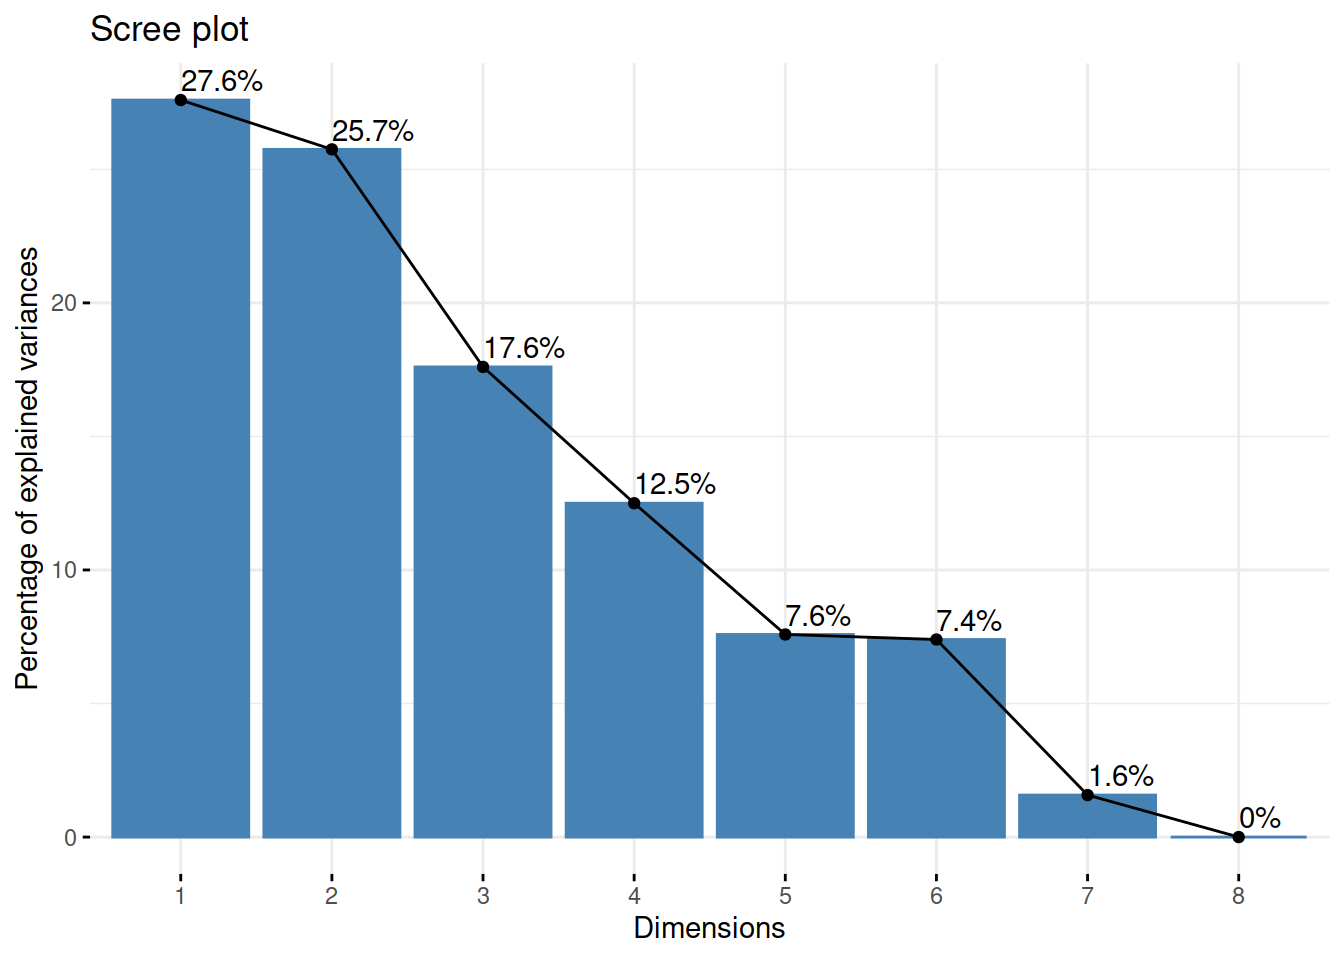
\includegraphics{Regresion_lineal_files/figure-latex/unnamed-chunk-4-1.pdf}

\hypertarget{regresion-lineal}{%
\section{Regresion Lineal}\label{regresion-lineal}}

\begin{Shaded}
\begin{Highlighting}[]
\NormalTok{model }\OtherTok{\textless{}{-}} \FunctionTok{lm}\NormalTok{(income  }\SpecialCharTok{\textasciitilde{}}\NormalTok{ education, }\AttributeTok{data =}\NormalTok{ df )}
\NormalTok{s }\OtherTok{=} \FunctionTok{summary}\NormalTok{(model)}
\NormalTok{s}
\end{Highlighting}
\end{Shaded}

\begin{verbatim}
## 
## Call:
## lm(formula = income ~ education, data = df)
## 
## Residuals:
##     Min      1Q  Median      3Q     Max 
## -39.572 -11.346  -1.501   9.669  53.740 
## 
## Coefficients:
##             Estimate Std. Error t value     Pr(>|t|)    
## (Intercept)  10.6035     5.1983   2.040       0.0475 *  
## education     0.5949     0.0863   6.893 0.0000000184 ***
## ---
## Signif. codes:  0 '***' 0.001 '**' 0.01 '*' 0.05 '.' 0.1 ' ' 1
## 
## Residual standard error: 17.04 on 43 degrees of freedom
## Multiple R-squared:  0.5249, Adjusted R-squared:  0.5139 
## F-statistic: 47.51 on 1 and 43 DF,  p-value: 0.0000000184
\end{verbatim}

\hypertarget{intervalos-de-confianza-para-ux3b20-y-ux3b21}{%
\section{Intervalos de confianza para β0 y
β1}\label{intervalos-de-confianza-para-ux3b20-y-ux3b21}}

Vemos los coefcientes y entre parentesis los intervalos de confianza
respectivos. La estimación de todo coeficiente de regresión tiene
asociada un error estándar, por lo tanto todo coeficiente de regresión
tiene su correspondiente intervalo de confianza.

\begin{Shaded}
\begin{Highlighting}[]
\NormalTok{model }\SpecialCharTok{\%\textgreater{}\%} 
\NormalTok{  pubh}\SpecialCharTok{::}\FunctionTok{glm\_coef}\NormalTok{()}
\end{Highlighting}
\end{Shaded}

\begin{verbatim}
##     Parameter        Coefficient Pr(>|t|)
## 1 (Intercept) 10.6 (0.12, 21.09)    0.048
## 2   education  0.59 (0.42, 0.77)  < 0.001
\end{verbatim}

\hypertarget{conclusiones}{%
\section{Conclusiones}\label{conclusiones}}

\begin{Shaded}
\begin{Highlighting}[]
\NormalTok{m\_output }\OtherTok{=} \FunctionTok{tidy}\NormalTok{(s, }\AttributeTok{conf.int =} \ConstantTok{TRUE}\NormalTok{)}
\NormalTok{m\_output}
\end{Highlighting}
\end{Shaded}

\begin{verbatim}
## # A tibble: 2 x 7
##   term        estimate std.error statistic      p.value conf.low conf.high
##   <chr>          <dbl>     <dbl>     <dbl>        <dbl>    <dbl>     <dbl>
## 1 (Intercept)   10.6      5.20        2.04 0.0475          0.120    21.1  
## 2 education      0.595    0.0863      6.89 0.0000000184    0.421     0.769
\end{verbatim}

\begin{Shaded}
\begin{Highlighting}[]
\NormalTok{s\_output }\OtherTok{=}\NormalTok{ broom}\SpecialCharTok{::}\FunctionTok{glance}\NormalTok{(s) }
\NormalTok{s\_output}
\end{Highlighting}
\end{Shaded}

\begin{verbatim}
## # A tibble: 1 x 8
##   r.squared adj.r.squared sigma statistic      p.value    df df.residual  nobs
##       <dbl>         <dbl> <dbl>     <dbl>        <dbl> <dbl>       <int> <dbl>
## 1     0.525         0.514  17.0      47.5 0.0000000184     1          43    45
\end{verbatim}

\begin{Shaded}
\begin{Highlighting}[]
\ControlFlowTok{if}\NormalTok{(s\_output}\SpecialCharTok{$}\NormalTok{p.value }\SpecialCharTok{\textgreater{}} \FloatTok{0.05}\NormalTok{)\{}\StringTok{"El p{-}value del estadístico F no es significativo para un α=0.05, luego el predictor no tiene asociación significativa sobre la variable respuesta"}\NormalTok{\}}\ControlFlowTok{else}\NormalTok{\{}\StringTok{"El p{-}value del estadístico F es significativo para un α=0.05, luego el predictor tiene asociación significativa con la variable respuesta, el modelo es útil."}\NormalTok{\}}
\end{Highlighting}
\end{Shaded}

\begin{verbatim}
## [1] "El p-value del estadístico F es significativo para un α=0.05, luego el predictor tiene asociación significativa con la variable respuesta, el modelo es útil."
\end{verbatim}

\begin{Shaded}
\begin{Highlighting}[]
\FunctionTok{paste0}\NormalTok{(}\StringTok{"Al tratarse de un modelo simple, el p{-}value de estadístico F es el mismo que el p{-}value del estadístico t del único predictor incluido en el modelo: "}\NormalTok{, m\_output}\SpecialCharTok{$}\NormalTok{term[}\DecValTok{2}\NormalTok{])}
\end{Highlighting}
\end{Shaded}

\begin{verbatim}
## [1] "Al tratarse de un modelo simple, el p-value de estadístico F es el mismo que el p-value del estadístico t del único predictor incluido en el modelo: education"
\end{verbatim}

\begin{Shaded}
\begin{Highlighting}[]
\FunctionTok{paste0}\NormalTok{(}\StringTok{"Residual standar error (RSE): En promedio, cualquier predicción del modelo se aleja "}\NormalTok{, }\FunctionTok{round}\NormalTok{(s\_output}\SpecialCharTok{$}\NormalTok{sigma, }\AttributeTok{digits =} \DecValTok{2}\NormalTok{),}\StringTok{" unidades del verdadero valor."}\NormalTok{)}
\end{Highlighting}
\end{Shaded}

\begin{verbatim}
## [1] "Residual standar error (RSE): En promedio, cualquier predicción del modelo se aleja 17.04 unidades del verdadero valor."
\end{verbatim}

\begin{Shaded}
\begin{Highlighting}[]
\FunctionTok{paste0}\NormalTok{(}\StringTok{"R2: El predictor \textquotesingle{}"}\NormalTok{, m\_output}\SpecialCharTok{$}\NormalTok{term[}\DecValTok{2}\NormalTok{], }\StringTok{"\textquotesingle{} empleado en el modelo es capaz de explicar el "}\NormalTok{, }\FunctionTok{round}\NormalTok{(s\_output}\SpecialCharTok{$}\NormalTok{r.squared}\SpecialCharTok{*}\DecValTok{100}\NormalTok{,}\AttributeTok{digits =} \DecValTok{2}\NormalTok{), }\StringTok{"\% de la variabilidad observada en los datos. La ventaja de R2 es que es independiente de la escala en la que se mida la variable respuesta, por lo que su interpretación es más sencilla."}\NormalTok{)}
\end{Highlighting}
\end{Shaded}

\begin{verbatim}
## [1] "R2: El predictor 'education' empleado en el modelo es capaz de explicar el 52.49% de la variabilidad observada en los datos. La ventaja de R2 es que es independiente de la escala en la que se mida la variable respuesta, por lo que su interpretación es más sencilla."
\end{verbatim}

\begin{Shaded}
\begin{Highlighting}[]
\FunctionTok{paste0}\NormalTok{(}\StringTok{"Intercepto (β0): El valor promedio de la variable respuesta cuando \textquotesingle{}"}\NormalTok{,m\_output}\SpecialCharTok{$}\NormalTok{term[}\DecValTok{2}\NormalTok{], }\StringTok{"\textquotesingle{} es 0 es de "}\NormalTok{, }\FunctionTok{round}\NormalTok{(m\_output}\SpecialCharTok{$}\NormalTok{estimate[}\DecValTok{1}\NormalTok{], }\AttributeTok{digits =} \DecValTok{2}\NormalTok{), }\StringTok{" unidades."}\NormalTok{)}
\end{Highlighting}
\end{Shaded}

\begin{verbatim}
## [1] "Intercepto (β0): El valor promedio de la variable respuesta cuando 'education' es 0 es de 10.6 unidades."
\end{verbatim}

\begin{Shaded}
\begin{Highlighting}[]
\ControlFlowTok{if}\NormalTok{(m\_output}\SpecialCharTok{$}\NormalTok{estimate[}\DecValTok{2}\NormalTok{] }\SpecialCharTok{\textgreater{}} \DecValTok{0}\NormalTok{)\{variacion }\OtherTok{=} \StringTok{"aumenta"}\NormalTok{\}}\ControlFlowTok{else}\NormalTok{\{variacion }\OtherTok{=} \StringTok{"disminuye"}\NormalTok{\}}
\FunctionTok{paste0}\NormalTok{(}\StringTok{"Predictor (β1): por cada unidad que se incrementa el predictor \textquotesingle{}"}\NormalTok{, m\_output}\SpecialCharTok{$}\NormalTok{term[}\DecValTok{2}\NormalTok{], }\StringTok{"\textquotesingle{} el valor de la variable respuesta \textquotesingle{}"}\NormalTok{, variacion, }\StringTok{"\textquotesingle{} en promedio "}\NormalTok{, }\FunctionTok{round}\NormalTok{(m\_output}\SpecialCharTok{$}\NormalTok{estimate[}\DecValTok{2}\NormalTok{], }\AttributeTok{digits =} \DecValTok{2}\NormalTok{), }\StringTok{" unidades."}\NormalTok{)}
\end{Highlighting}
\end{Shaded}

\begin{verbatim}
## [1] "Predictor (β1): por cada unidad que se incrementa el predictor 'education' el valor de la variable respuesta 'aumenta' en promedio 0.59 unidades."
\end{verbatim}

\hypertarget{ecuaciuxf3n-del-modelo}{%
\subsection{ecuación del modelo}\label{ecuaciuxf3n-del-modelo}}

\begin{Shaded}
\begin{Highlighting}[]
\NormalTok{beta\_0 }\OtherTok{=}\NormalTok{ model}\SpecialCharTok{$}\NormalTok{coefficients[[}\DecValTok{1}\NormalTok{]]}
\NormalTok{beta\_1 }\OtherTok{=}\NormalTok{ model}\SpecialCharTok{$}\NormalTok{coefficients[[}\DecValTok{2}\NormalTok{]]}
\FunctionTok{paste0}\NormalTok{(}\StringTok{"La ecuación lineal de regresión sería:  Y = "}\NormalTok{, }\FunctionTok{round}\NormalTok{(beta\_0, }\AttributeTok{digits =} \DecValTok{2}\NormalTok{), }\StringTok{" + "}\NormalTok{,}\FunctionTok{round}\NormalTok{(beta\_1, }\AttributeTok{digits =} \DecValTok{2}\NormalTok{), }\StringTok{" * X + E"}\NormalTok{)}
\end{Highlighting}
\end{Shaded}

\begin{verbatim}
## [1] "La ecuación lineal de regresión sería:  Y = 10.6 + 0.59 * X + E"
\end{verbatim}

\hypertarget{estimaciuxf3n-para-un-valor-particular.}{%
\section{Estimación para un valor
particular.}\label{estimaciuxf3n-para-un-valor-particular.}}

\begin{Shaded}
\begin{Highlighting}[]
\NormalTok{nuevo}\OtherTok{\textless{}{-}}\FunctionTok{data.frame}\NormalTok{(}\AttributeTok{education=}\DecValTok{80}\NormalTok{)}
\FunctionTok{predict.lm}\NormalTok{(model,}\AttributeTok{newdata=}\NormalTok{nuevo)}
\end{Highlighting}
\end{Shaded}

\begin{verbatim}
##        1 
## 58.19225
\end{verbatim}

\hypertarget{diagnuxf3sticos-del-modelo-lineal}{%
\section{Diagnósticos del modelo
lineal}\label{diagnuxf3sticos-del-modelo-lineal}}

Una de las mejores formas de confirmar que las condiciones necesarias
para un modelo de regresión lineal simple por mínimos cuadrados se
cumplen es mediante el estudio de los residuos del modelo.

En R, los residuos se almacenan dentro del modelo bajo el nombre de
residuals. R genera automáticamente los gráficos más típicos para la
evaluación de los residuos de un modelo.

\begin{Shaded}
\begin{Highlighting}[]
\FunctionTok{library}\NormalTok{(ggfortify)}
\FunctionTok{autoplot}\NormalTok{(model)}
\end{Highlighting}
\end{Shaded}

\includegraphics{Regresion_lineal_files/figure-latex/unnamed-chunk-10-1.pdf}
Los residuos confirman que los datos no se distribuyen de forma lineal,
ni su varianza constante (plot1). Además se observa que la distribución
de los residuos no es normal (plot2). Algunas observaciones tienen un
residuo estandarizado absoluto mayor de 3 (1.73 si se considera la raíz
cuadrada) lo que es indicativo de observación atípica (plot3). Valores
de Leverages (hat) mayores que 2.5x((p+1)/n), siendo p el número de
predictores y n el número de observaciones, o valores de Cook mayores de
1 se consideran influyentes (plot4). Todo ello reduce en gran medida la
robustez de la estimación del error estándar de los coeficientes de
correlación estimados y con ello la del modelo es su conjunto.

\hypertarget{datos-outliers}{%
\section{Datos outliers}\label{datos-outliers}}

\begin{Shaded}
\begin{Highlighting}[]
\NormalTok{model }\SpecialCharTok{\%\textgreater{}\%}\NormalTok{ olsrr}\SpecialCharTok{::}\FunctionTok{ols\_plot\_cooksd\_bar}\NormalTok{()}
\end{Highlighting}
\end{Shaded}

\includegraphics{Regresion_lineal_files/figure-latex/unnamed-chunk-11-1.pdf}

\hypertarget{outliers-o-puntos-con-alta-influencia}{%
\section{Outliers o puntos con alta
influencia}\label{outliers-o-puntos-con-alta-influencia}}

Otra forma de identificar las observaciones que puedan ser outliers o
puntos con alta influencia (leverage) es emplear las funciones
rstudent() y hatvalues().

\begin{Shaded}
\begin{Highlighting}[]
\FunctionTok{plot}\NormalTok{(}\AttributeTok{x =}\NormalTok{ model}\SpecialCharTok{$}\NormalTok{fitted.values, }\AttributeTok{y =} \FunctionTok{abs}\NormalTok{(}\FunctionTok{rstudent}\NormalTok{(model)),}
     \AttributeTok{main =} \StringTok{"Absolute studentized residuals vs predicted values"}\NormalTok{, }\AttributeTok{pch =} \DecValTok{20}\NormalTok{,}
     \AttributeTok{col =} \StringTok{"grey30"}\NormalTok{)}
\FunctionTok{abline}\NormalTok{(}\AttributeTok{h =} \DecValTok{3}\NormalTok{, }\AttributeTok{col =} \StringTok{"red"}\NormalTok{)}
\end{Highlighting}
\end{Shaded}

\includegraphics{Regresion_lineal_files/figure-latex/unnamed-chunk-12-1.pdf}

En este caso muchos de los valores parecen posibles outliers o puntos
con alta influencia porque los datos realmente no se distribuyen de
forma lineal en los extremos.

\hypertarget{normalidad-en-los-residuos}{%
\section{Normalidad en los residuos}\label{normalidad-en-los-residuos}}

\begin{Shaded}
\begin{Highlighting}[]
\NormalTok{jtools}\SpecialCharTok{::}\FunctionTok{plot\_summs}\NormalTok{(model, }\AttributeTok{plot.distributions =} \ConstantTok{TRUE}\NormalTok{, }\AttributeTok{inner\_ci\_level =}\NormalTok{ .}\DecValTok{9}\NormalTok{)}
\end{Highlighting}
\end{Shaded}

\includegraphics{Regresion_lineal_files/figure-latex/unnamed-chunk-13-1.pdf}

\pagebreak

\hypertarget{resumen-del-modelo-lineal}{%
\subsection{resumen del modelo lineal}\label{resumen-del-modelo-lineal}}

\begin{Shaded}
\begin{Highlighting}[]
\NormalTok{model }\SpecialCharTok{\%\textgreater{}\%}\NormalTok{ broom}\SpecialCharTok{::}\FunctionTok{augment}\NormalTok{() }\SpecialCharTok{\%\textgreater{}\%} \FunctionTok{as\_tibble}\NormalTok{() }\SpecialCharTok{\%\textgreater{}\%} \FunctionTok{head}\NormalTok{()}
\end{Highlighting}
\end{Shaded}

\begin{verbatim}
## # A tibble: 6 x 9
##   .rownames  income education .fitted  .resid   .hat .sigma    .cooksd .std.re~1
##   <chr>       <int>     <int>   <dbl>   <dbl>  <dbl>  <dbl>      <dbl>     <dbl>
## 1 accountant     62        86    61.8   0.239 0.0509   17.2 0.00000554    0.0144
## 2 pilot          72        76    55.8  16.2   0.0363   17.0 0.0177        0.968 
## 3 architect      75        92    65.3   9.67  0.0621   17.2 0.0114        0.586 
## 4 author         55        90    64.1  -9.14  0.0582   17.2 0.00944      -0.553 
## 5 chemist        64        86    61.8   2.24  0.0509   17.2 0.000488      0.135 
## 6 minister       21        84    60.6 -39.6   0.0476   16.1 0.142        -2.38  
## # ... with abbreviated variable name 1: .std.resid
\end{verbatim}

\hypertarget{graficos-de-regresion}{%
\subsection{Graficos de Regresion}\label{graficos-de-regresion}}

\begin{Shaded}
\begin{Highlighting}[]
\NormalTok{ggpubr}\SpecialCharTok{::}\FunctionTok{ggscatter}\NormalTok{(df, }\AttributeTok{x =} \StringTok{"income"}\NormalTok{, }\AttributeTok{y =} \StringTok{"education"}\NormalTok{,}
   \CommentTok{\#color = "black", shape = 21, size = 3, \# Points color, shape and size}
   \AttributeTok{add =} \StringTok{"reg.line"}\NormalTok{,  }\CommentTok{\# Add regressin line}
   \AttributeTok{add.params =} \FunctionTok{list}\NormalTok{(}\AttributeTok{color =} \StringTok{"blue"}\NormalTok{, }\AttributeTok{fill =} \StringTok{"lightgray"}\NormalTok{), }\CommentTok{\# Customize reg. line}
   \AttributeTok{conf.int =} \ConstantTok{TRUE}\NormalTok{, }\CommentTok{\# Add confidence interval}
   \AttributeTok{cor.coef =} \ConstantTok{TRUE}\NormalTok{, }\CommentTok{\# Add correlation coefficient. see ?stat\_cor}
   \AttributeTok{cor.coeff.args =} \FunctionTok{list}\NormalTok{(}\AttributeTok{method =} \StringTok{"pearson"}\NormalTok{, }\AttributeTok{label.x =} \DecValTok{3}\NormalTok{, }\AttributeTok{label.sep =} \StringTok{"}\SpecialCharTok{\textbackslash{}n}\StringTok{"}\NormalTok{)}
\NormalTok{   )}
\end{Highlighting}
\end{Shaded}

\includegraphics{Regresion_lineal_files/figure-latex/unnamed-chunk-15-1.pdf}

\hypertarget{grafico-con-intervalo-de-confianza-e-intervalo-de-predicciuxf3n}{%
\subsection{Grafico con Intervalo de confianza e intervalo de
predicción}\label{grafico-con-intervalo-de-confianza-e-intervalo-de-predicciuxf3n}}

Como es de esperar ambos intervalos están centrados en torno al mismo
valor. Si bien ambos parecen similares, la diferencia se encuentra en
que los intervalos de confianza se aplican al valor promedio que se
espera de y para un determinado valor de x, mientras que los intervalos
de predicción no se aplican al promedio. Por esta razón, los segundos
siempre son más amplios que los primeros.

\begin{Shaded}
\begin{Highlighting}[]
\NormalTok{res.predict }\OtherTok{=} \FunctionTok{predict}\NormalTok{(model, }\AttributeTok{interval =} \StringTok{"prediction"}\NormalTok{)}
\NormalTok{res.predict}
\end{Highlighting}
\end{Shaded}

\begin{verbatim}
##                         fit        lwr       upr
## accountant         61.76141  26.539316  96.98350
## pilot              55.81282  20.836201  90.78943
## architect          65.33057  29.920918 100.74022
## author             64.14085  28.797035  99.48466
## chemist            61.76141  26.539316  96.98350
## minister           60.57169  25.405447  95.73794
## professor          65.92543  30.481623 101.36923
## dentist            70.08944  34.383715 105.79517
## reporter           62.35627  27.104996  97.60754
## engineer           61.76141  26.539316  96.98350
## undertaker         54.62310  19.685380  89.56081
## lawyer             68.89972  33.272886 104.52656
## physician          68.30486  32.716260 103.89347
## welfare.worker     60.57169  25.405447  95.73794
## teacher            64.73571  29.359389 100.11203
## conductor          30.82872  -4.058868  65.71631
## contractor         37.37217   2.609500  72.13485
## factory.owner      43.91563   9.172662  78.65859
## store.manager      36.77731   2.007621  71.54701
## banker             59.38197  24.268215  94.49573
## bookkeeper         53.43338  18.531130  88.33563
## mail.carrier       43.32077   8.580369  78.06117
## insurance.agent    52.83852  17.952716  87.72432
## store.clerk        40.34647   5.605830  75.08711
## carpenter          24.28527 -10.831320  59.40185
## electrician        33.80302  -1.014800  68.62083
## RR.engineer        27.25956  -7.740139  62.25926
## machinist          29.63900  -5.282529  64.56053
## auto.repairman     23.69041 -11.452095  58.83291
## plumber            25.47498  -9.592303  60.54227
## gas.stn.attendant  27.85442  -7.124454  62.83330
## coal.miner         14.76751 -20.863621  50.39865
## streetcar.motorman 26.06984  -8.974065  61.11375
## taxi.driver        21.90583 -13.319467  57.13112
## truck.driver       19.52639 -15.820994  54.87377
## machine.operator   22.50069 -12.696171  57.69755
## barber             26.06984  -8.974065  61.11375
## bartender          27.25956  -7.740139  62.25926
## shoe.shiner        20.71611 -14.568566  56.00078
## cook               23.69041 -11.452095  58.83291
## soda.clerk         28.44928  -6.509623  63.40819
## watchman           25.47498  -9.592303  60.54227
## janitor            22.50069 -12.696171  57.69755
## policeman          38.56189   3.810645  73.31314
## waiter             29.63900  -5.282529  64.56053
\end{verbatim}

\begin{Shaded}
\begin{Highlighting}[]
\NormalTok{df }\OtherTok{=} \FunctionTok{bind\_cols}\NormalTok{(Duncan, res.predict)}

\NormalTok{df }\SpecialCharTok{\%\textgreater{}\%} 
  \FunctionTok{ggplot}\NormalTok{(}\FunctionTok{aes}\NormalTok{(}\AttributeTok{x=}\NormalTok{education, }\AttributeTok{y=}\NormalTok{income))}\SpecialCharTok{+}
  \FunctionTok{geom\_point}\NormalTok{()}\SpecialCharTok{+}
  \FunctionTok{geom\_line}\NormalTok{(}\FunctionTok{aes}\NormalTok{(}\AttributeTok{y=}\NormalTok{lwr), }\AttributeTok{color =} \StringTok{"red"}\NormalTok{, }\AttributeTok{linetype =} \StringTok{"dashed"}\NormalTok{)}\SpecialCharTok{+}
  \FunctionTok{geom\_line}\NormalTok{(}\FunctionTok{aes}\NormalTok{(}\AttributeTok{y=}\NormalTok{upr), }\AttributeTok{color =} \StringTok{"red"}\NormalTok{, }\AttributeTok{linetype =} \StringTok{"dashed"}\NormalTok{)}\SpecialCharTok{+}
  \FunctionTok{geom\_smooth}\NormalTok{(}\AttributeTok{method=}\NormalTok{lm, }\AttributeTok{se=}\ConstantTok{TRUE}\NormalTok{) }
\end{Highlighting}
\end{Shaded}

\includegraphics{Regresion_lineal_files/figure-latex/unnamed-chunk-16-1.pdf}

\hypertarget{test-sobre-normalidad-de-residuos}{%
\subsection{Test sobre Normalidad de
Residuos}\label{test-sobre-normalidad-de-residuos}}

\begin{Shaded}
\begin{Highlighting}[]
\NormalTok{residuos}\OtherTok{\textless{}{-}}\FunctionTok{resid}\NormalTok{(model)}
\FunctionTok{ks.test}\NormalTok{(residuos,}\StringTok{"pnorm"}\NormalTok{)}
\end{Highlighting}
\end{Shaded}

\begin{verbatim}
## 
##  Exact one-sample Kolmogorov-Smirnov test
## 
## data:  residuos
## D = 0.44439, p-value = 0.00000001283
## alternative hypothesis: two-sided
\end{verbatim}

\begin{Shaded}
\begin{Highlighting}[]
\FunctionTok{qqnorm}\NormalTok{(residuos)}
\FunctionTok{qqline}\NormalTok{(residuos)}
\end{Highlighting}
\end{Shaded}

\includegraphics{Regresion_lineal_files/figure-latex/unnamed-chunk-18-1.pdf}
\#\# Anoval del modelo

\begin{Shaded}
\begin{Highlighting}[]
\FunctionTok{anova}\NormalTok{(model)}
\end{Highlighting}
\end{Shaded}

\begin{verbatim}
## Analysis of Variance Table
## 
## Response: income
##           Df Sum Sq Mean Sq F value       Pr(>F)    
## education  1  13790 13790.2  47.511 0.0000000184 ***
## Residuals 43  12481   290.3                         
## ---
## Signif. codes:  0 '***' 0.001 '**' 0.01 '*' 0.05 '.' 0.1 ' ' 1
\end{verbatim}

\end{document}
